\section{उच्चारण}\label{sec:intro-pronounce}\index{उच्चारण}
हिन्दी की तरह, रूसी भाषा में भी अधिकतर जैसा लिखते हैं वैसा ही बोलते हैं। परंतु इसमे कुछ अपवाद भी हैं, प्रधानत:
\begin{itemize}
    \item \ru{его} को लिखते \textit{यगो} हैं परंतु बोलते \textit{यवो} हैं
    \item \ru{--ого} को लिखते \textit{ओगो} हैं परंतु बोलते \textit{ओवो} हैं, यह शब्द प्राय: उपसर्ग (suffix) में होता है।
    \item \ru{что} को लिखते \textit{च्तो} हैं पर पढ़ते ष्तो हैं। इसी तरह बहुत ऐसे शब्द हैं जहां \ru{ч} का उच्चारण ष कि तरह होता है।
\end{itemize}

रूसी शब्दों के उच्चारण मे यह बहुत महत्वपूर्ण है कि शब्द के किस भाग पर बल दिया जा रहा है, उदाहरत:
\begin{itemize}
    \item \ru{ст\'оит} [उच्चारण: स्तोइत; धातु: \ru{стоять}] का अर्थ किसी वस्तु, व्यक्ति, अथवा जन्तु के खड़े होने से
    है। \par उदाहरण के लिए: \ru{он стоит там} $\rightarrow$ वह वहाँ खड़ा है।
    \item \ru{сто\'ит} [उच्चारण: स्तईत; धातु: \ru{стоить}] का अर्थ पैसा अथवा किसी वस्तु का मूल्य होता है| \par उदाहरण के लिए: \ru{сколько стоит} $\rightarrow$ कितना मूल्य है।
\end{itemize}

इसी प्रकार~\cite{levine2009}:
\begin{itemize}
    \item \ru{мук\'а}\index{\ru{мук\'а}} [उच्चारण: मुका] का अर्थ आटा है, और,
    \item \ru{м\'ука}\index{\ru{м\'ука}} [उच्चारण: मूका] का अर्थ दु:ख, दर्द, अथवा प्रताड़ना है।
\end{itemize}

इसी कारण कई पुस्तकों में शब्द के जिस अक्षर पर बल देना हो, उसे accent {\color{blue} {\large $\left( \acute{\,}\, \right)$}} से चिन्हित किया गया होता है। % Latex -> \, => small space in maths mode

\subsection{\sru{ъ}, \sru{ь}, तथा \sru{ы} का उच्चारण}\label{subsec:alpha-pronounce-special-char}

\ru{ъ} और \sru{ь} उच्चारण के अक्षर हैं और इनका अलग से उच्चारण नहीं होता है, यह दोनों अक्षर जिस शब्द के आगे लगते हैं उन पर कम या ज़्यादा बल देना होता
है। इन्ही कारणों से इन्हे \ru{твёрди знак}, \ru{твёрди} = कठोर, और \ru{мякий знак}, \ru{мякий} = कोमल, \ru{знак} = चिन्ह कहा जाता है।

\subsubsection{\sru{ъ}: \sru{твёрди знак}: [त्वयोरदी ज़्नाक]}\label{subsubsec:alpha-pronounce-special-char-hard}\index{\ru{твёрди знак}}
इसे कठोर चिन्ह कहते हैं, इसका कोई अलग से उच्चारण नहीं है, यह जिस अक्षर के आगे लगता है उस पर बल देना होता है। यह संस्कृत भाषा के s चिन्ह कि तरह है। उदाहरण के लिए:
\begin{itemize}
    \item \ru{съезд}\index{\ru{съезд}} $\rightarrow$
    \item \ru{съесть}\index{\ru{съесть}} $\rightarrow$
    \item \ru{объявить}\index{\ru{объявить}} $\rightarrow$
    \item \ru{объëму}\index{\ru{объëму}} $\rightarrow$
    \item \ru{съëмки}\index{\ru{съëмки}} $\rightarrow$
\end{itemize}

यह अक्षर 1917 से पहले लगभग हर शब्द के अंत मे लगता था, परंतु 1917 के क्रांतिकारी तख्तापलट के पशच्यात इसे खतम कर दिया गया। इस अक्षर का प्रयोग दो शब्दों को विभाजित
करने के लिए भी होता था~\cite{guzeva2020}।

%% Insert diagram here

\subsubsection{\sru{ь}: \sru{мякий знак}: [म्याकि ज़्नाक]}\label{subsubsec:alpha-pronounce-special-char-soft}\index{\ru{мякий знак}}
यह कोमल उच्चारण का चिन्ह है, हिन्दी/संस्कृत के हलंत की तरह उच्चारण होना चाहिए, परंतु कई बार ये ऐसे अक्षरों के आगे भी लग जाता है जिनके आगे प्राय: हिन्दी या संस्कृत में
हलंत नहीं लगाते। यह चिन्ह जिस अक्षर के आगे लगता है, उच्चारण के समय के समय जिह्वा ऊपर के आगे के दांतों को छू रही होती है। जैसे \ru{брать} [ब्रात] (भ्राता/भाई) में `त्'
को उच्चारित करने के लिए `त' बोलते समय जिह्वा ऊपर के मुख के सामने के दांतों को पीछे कि तरफ से छूती है। इसे \ref{fig:intro-pronounce-soft} में दर्शाया गया है।

\begin{figure}
    \label{fig:intro-pronounce-soft}

    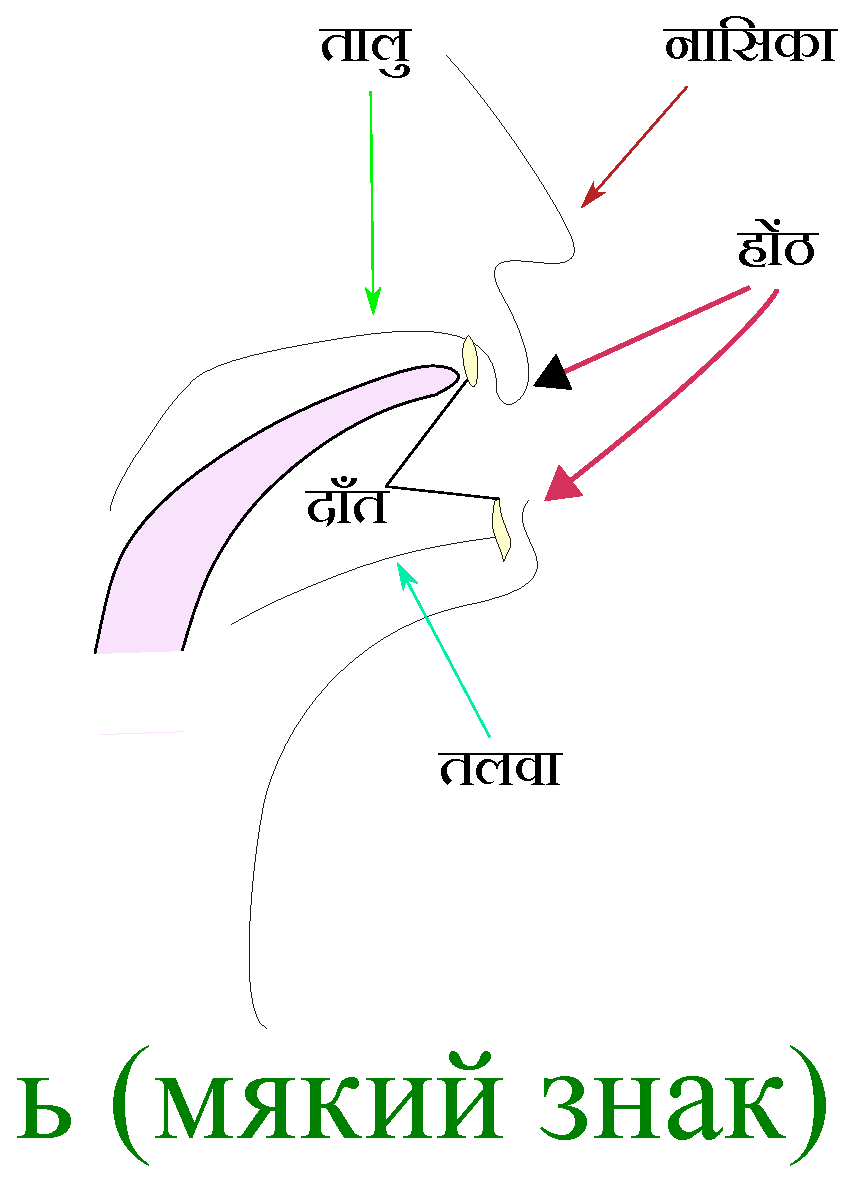
\includegraphics[scale=0.35]{graphics/pronounce-soft}
    \caption{\ru{ь} का उच्चारण}

\end{figure}

\subsubsection{\sru{ы}}\label{subsubsec:alpha-pronounce-special-char-oui}\index{\ru{ы}}
इसे `ऋ' अक्षर में अगर `र' की ध्वनि निकाल दी जाए, और अंत के `ई' के जैसे उच्चारित करते हैं। संस्कृत भाषा में
ऐसे अक्षरों को जिह्वामूलीय अक्षर कहते हैं, जहां ध्वनि जिव्हा की जड़ से निकलती है, और जिह्वा स्वय: मुँह के
बीच में रहती है, न ऊपर न नीचे के दांतों को छूती ह~\cite{macdonald1926}। इसे~\ref{fig:intro-pronounce-oui} में दर्शाया गया है।
उच्चारण के लिए \href{https://www .youtube .com/watch?v=s6asiEL1f8U}{यह विडिओ}~\cite{kovalenko2015} देखिए।
\begin{figure}
    \label{fig:intro-pronounce-oui}
    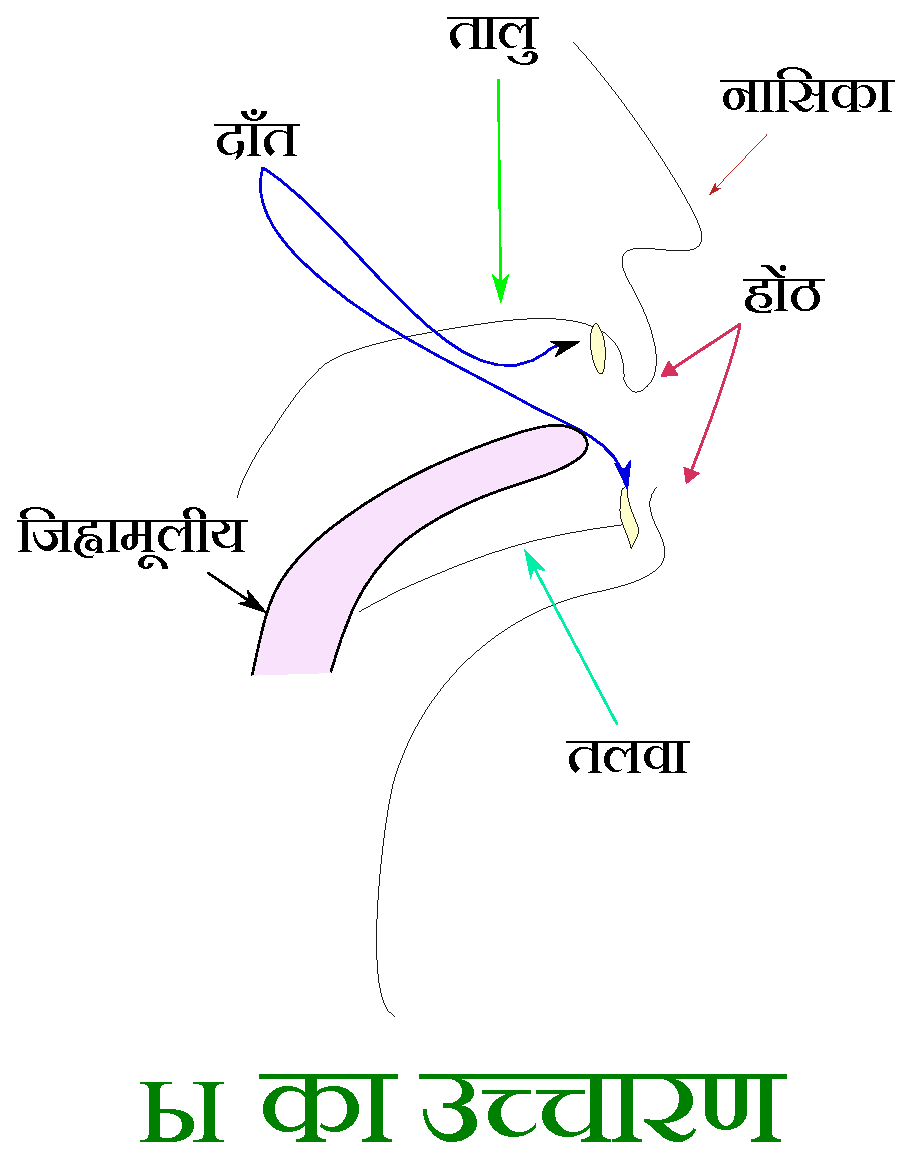
\includegraphics[scale=0.35]{graphics/pronounce-oui}
    \caption{\ru{ы} का उच्चारण}
\end{figure}
